\documentclass[a4paper,14pt]{report}
\usepackage[utf8]{inputenc}
\usepackage[T1]{fontenc}
\usepackage{titlesec}
\usepackage{float}
\usepackage{graphicx}
\graphicspath{ {./wykresy/} }

\renewcommand{\contentsname}{Spis treści}

\titleformat{\chapter}[display]
  {\normalfont\bfseries}{}{0pt}{\Huge}

\usepackage{pgfplots}
 
\pgfplotsset{compat = newest}

\title{Obliczenia naukowe Lista 3}
\author{Radosław Wojtczak}
\date{Numer indeksu: 254607}
\begin{document}
\maketitle
\tableofcontents


\section{Wstęp do zadań 1-3}
  Główny celem zadań 1-3 było zaimplementowanie podanych przez Pana Profesora funkcji mających na celu szukanie odpowiedniego $r \in R$ dla którego zadana funkcja $f:R->R$ przyjmuje wartość 0 ($f(r)=0$). Ze względu na wykonywanie obliczeń w skończonych arytmetykach (warunkowanych faktem, iż pamięc w komputerach jest skończona) otrzymane wyniki są na ogół przybliżone, jednak dokładność obliczeń może być z góry określona i dobiera się ją zależnie od potrzeb. (co oznacza, że nie sprawdzamy tak jak w modelu, czy coś jest równe 0, tylko czy otrzymany wynik jest dostatecznie bliski zera. Pojęcie "bliskość" zależy od ustalonych dokładności). Głównym obiektem badań będą funkcję nieliniowe, gdyż wyszukiwanie zer w funkcjach liniowych jest zadaniem trywialnym. \\
  Wszystkie implementacje metod znajdują się w pliku \textit{header.jl} w module \textit{Functions}. Dodatkowo plik \textit{tests.jl} odpowiada za testowanie zaimplementowanych funkcji.
\chapter{Zadanie 1.}
  \section{Wstęp}
  Pierwszą z funkcji jest funkcja, której działanie opiera się na metodzie bisekcji (metodzie połowienia), której ideą jest dzielenie początkowego przedziału na coraz to mniejsze, w celu znalezienia odpowiedniego przybliżenia miejsca zerowego funkcji. 
  \section{Opis algorytmu}
  Swoje działanie ów metoda opiera na \textit{twierdzeniu Darboux} (które poznaliśmy na analizie matematycznej w trakcie pierwszego roku studiów). Mówiąc kolokwialnie, jeśli funkcja na końcach wybranego przez nas przedziału ma inny znak i jest ciągła, to znaczy, że w którymś momencie "musiała zmienić znak", to znaczy znaleźć się w punkcie $y=0$, czyli w miejscu zerowym. Od razu zauważamy, że możliwość użycia tej metody jest warunkowana przez ciągłość funkcji, jak i wybranie przedziału na którego końcach funkcja przyjmuje wartości o różnych znakach. Następnie dzielimy przedział na pół (\textbf{UWAGA: } środek przedziału nie jest obliczany w sposób $\frac{(a+b)}{2}$ ze względu na to, iż w pewnych przypadkach możemy paradoksalnie otrzymać liczbę spoza rozpatrywanego przedziału. Z tego względu środek obliczany jest w następujący sposób: $a+\frac{(b-a)}{2}$ ) i sprawdzamy w której części dalej zachodzi warunek różnych znaków na końcach. Dokonujemy ów podziału do momentu, aż wyznaczony środek podstawiony pod funkcję f zwraca wynik równy 0( oczywiście, ze względu na ograniczenia sprzętowe nie sprawdzamy, czy otrzymana wartość to dokładnie zero- tutaj wprowadzamy takie pojęcia jak \textit{delta} czy \textit{epsilon}, które informują nas z jaką dokładnością poszukujemy zadanego pierwiastka funkcji).
  Warunkiem zakończenia pracy algorytmu jest znalezienie takiej wartości $r$ dla której $f(r)=0$ (z dokładnością do \textit{epsilon}) lub niemożliwość podziału zadanego przedziału na mniejsze (co warunkuje parametr \textit{delta}).

\chapter{Zadanie 2.}
  \section{Wstęp}
  Drugą z funkcji jest funkcja, której działanie opiera się na metodzie stycznych(zwanej również metodą \textit{Newtona}), której ideą jest wykorzystanie pojęcia stycznej w celu znalezienia odpowiedniego przybliżenia pierwiastka równania.
  \section{Opis algorytmu}
  Wybieramy punkt początkowy $x_{0}$ i konstruujemy styczną do funkcji w punkcie $x_{0}$. W wyniku tej operacji ów styczna przecina oś OX w punkcie $x_{1}$, który będzie następnym przybliżeniem miejsca zerowego. Następnie powtarzamy powyższy proces aż do momentu, gdy otrzymany wynik jest dostatecznie bliski zera (warunkowane parametrem \textit{epsilon}), odległość między przybliżeniami jest zbyt bliska (warunkowane parametrem \textit{delta}) lub liczba iteracji wykracza poza zakres (liczba iteracji determinowana jest przez parametr \textit{maxit}).
  Aby powyższy algorytm zadziałał muszą zostać spełnione następujące własności:
  \begin{itemize}
    \item Wyszukiwany pierwiastek jest pierwiastkiem jednokrotnym (bez odpowiednich modyfikacji przy rowiązywaniu równań zawierających pierwiastki wielokrotne metoda Newtona może być dużo wolniejsza niż inne metody rozwiązywania równań)
    \item Pierwsza i druga pochodna muszą mieć stały znak w przedziale
    \item Funkcja musi mieć różne znaki na końcach rozpatrywanego przedziału
  \end{itemize}
  Ze względu na wykorzystanie pojęcia stycznej, które jest związane z pojęciem pochodnej(styczną możemy traktować jako geometryczną interpretację pochodnej funkcji), szybko zauważamy, iż wadą ów metody jest potrzeba obliczania pochodnej funkcji.
\chapter{Zadanie 3.}
  \section{Wstęp}
  Ostatnią z funkcji jest funkcja, której działanie opiera się na metodzie siecznych (zwanej również metodą \textit{Eulera}), której ideą jest wykorzystanie pojęcia siecznej (prostej przecinającej daną krzywą[tu:wykres funkcji] w co najmniej dwóch punktach) w celu znalezienia odpowiedniego przybliżenia pierwiastka równania.
  \section{Opis algorytmu}
  Ta metoda jest drobną modyfikacją metody Newtona- zamiast wykorzystywać pochodną, dokonujemy jej aproksymacji przy pomocy ilorazu różnicowego (oczywiście ów ułatwienie spowoduje, iż ta metoda nie zawsze będzie zbieżna).
  Wybieramy dwa punkty startowe- $x_{0}$ oraz $x_{1}$. Konstruujemy sieczną, której przecięcie z osią OX jest kolejnym przybliżeniem miejsca zerowego (dla przykładu niech ów miejsce będzie równe $x_{2}$). Następnie powtarzamy procedurę: dla $x_{1}$ i $x_{2}$, $x_{2}$ i $x_{3}$ i tak dalej, aż do momentu, gdy otrzymany wynik jest dostatecznie bliski zera (warunkowane parametrem \textit{epsilon}), odległość między przybliżeniami jest zbyt bliska (warunkowane parametrem \textit{delta}) lub liczba iteracji wykracza poza zakres (liczba iteracji determinowana jest przez parametr \textit{maxit}).
  Aby powyższy algorytm zadziałał muszą zostać spełnione następujące własności:
  \begin{itemize}
    \item Funkcja jest określona w przedziale $[a,b]$
    \item Funkcja jest ciągła w przedziale $[a,b]$
    \item Na krańcach przedziału $[a,b]$ funkcja ma różne znaki
    \item W przedziale $[a,b]$ pierwsza pochodna funkcji jest różna od zera
  \end{itemize}

\chapter{Zadanie 4.}
  \section{Krótki opis problemu}
  Dla zadanej funkcji
  \begin{equation}
    f(x)=sin(x)-(\frac{1}{2}*x)^{2}
  \end{equation}
  należało znaleźć miejsca zerowe funkcji przy pomocy wcześniej zaimplementowanych metod.
  \section{Rozwiązanie}
  Rozwiązanie znajdujące się w pliku \textbf{zad4.jl} polega na dosłownej implementacji funkcji podanej w treści zadania oraz sprawdzeniu dla niej przybliżonych miejsc zerowych z podanymi parametrami.\\
  Korzystając z narzędzi matematycznych dostępnych do publicznego użytku spodziewamy się, iż ów miejscem zerowym w wyznaczonym przedziale będzie $x\approx 1.93375$.
  \section{Wyniki oraz ich interpretacje}
  Poniższa tabela przedstawia wyniki otrzymane w ramach uruchomienia pliku \textbf{zad4.jl} \\
  \begin{table}[H]
    \centering
    \begin{tabular}{|c | c | c | c |} 
     \hline
     Algorytm & r & $f(r)$ & Liczba iteracji \\ [0.5ex] 
     \hline\hline
     Metoda bisekcji & 1.9337539672851562 & -2.7027680138402843e-7 & 16  \\ 
     Metoda stycznych & 1.933753779789742 & -2.2423316314856834e-8 & 4\\
     Metoda siecznych & 1.933753644474301 & 1.564525129449379e-7 & 4\\
     \hline
    \end{tabular}
    \caption{Otrzymane przybliżenia miejsc zerowych}
    \label{Zad4Wyniki}
    \end{table}
    \textbf{Interpretacja: }Zauważamy, iż dla żadnej z ów metod wartość $f(r)$ nie jest dokładnie równa 0 (czego z perspektywy teorii matematycznej powinniśmy się spodziewać), jednakże wynika to z faktu użycia odpowiednich parametrów określających poprawność rozwiązania. Na tej podstawie wnioskujemy, iż otrzymany wynik jest jedynie przybliżeniem miejsca zerowego rozpatrywanej funkcji, jednak każda z powyższych metod była w stanie zwrócić satysfakcjonujące przybliżenie. Dodatkowo zauważamy, iż metoda bisekcji potrzebowała 2 razy więcej wywołań niż metoda stycznych czy siecznych, aby rozwiązać otrzymany problem.
  \section{Wnioski}
    Przy odpowiednich danych początkowych każdy z algorytmów produkuje poprawne rozwiązania z dokładnością do ustalonych parametrów, jednakże ów rozwiązania różnia się liczbą iteracji potrzebną do uzyskania oczekiwanego wyniku, co wynika z różnic w zbieżności między wykorzystanymi metodami.
\chapter{Zadanie 5.}
  \section{Krótki opis problemu}
    Naszym zadaniem było znalezienie punktów przecięcia funkcji $y=3x$ z funkcją $y=e^{x}$. Następnie przy pomocy metody bisekcji mieliśmy znaleźć odpowiednie przybliżenie miejsca zerowego uzyskanej funkcji.
  \section{Rozwiązanie}
    W celu wyznaczenia odpowiedniego równania przeprowadzamy następujący szereg przekształceń
    $y=y$ \textbf{---->} $e^{x}=3*x$ \textbf{---->} $e^{x}-3*x=0 $.\\
    Następnie przy pomocy dostępnych narzędzi matematycznych obliczamy miejsca zerowe otrzymanej funkcji: są to $x_{1} \approx 0.619061$ i $x_{2} \approx 1.51213 $. Dzięki tej wiedzy jesteśmy w stanie odpowiednio spreparować rozpatrywane przedziały. \\
    W pliku \textbf{zad5.jl} znajduje się implementacja powyższego rozumowania. 
    \begin{figure}[H]
      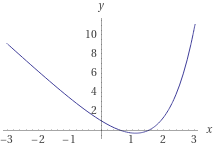
\includegraphics[scale=1.0]{zad5}
      \centering
      \caption{Wykres funkcji $e^{x}-3*x$}
    \end{figure}
  \section{Wyniki oraz ich interpretacje}
    Poniższa tabela przedstawia wyniki otrzymane w ramach uruchomienia pliku \textbf{zad5.jl} \\

    \begin{table}[H]
    \centering
    \begin{tabular}{|c | c | c | c |} 
     \hline
     Przedział & r & $f(r)$ & Liczba iteracji \\ [0.5ex] 
     \hline\hline
     $[0,1]$ & 0.619140625 & -9.066320343276146e-5 & 9  \\ 
     $[1,2]$ & 1.5120849609375 & -7.618578602741621e-5 & 13 \\
     \hline
    \end{tabular}
    \caption{Otrzymane przybliżenia miejsc zerowych}
    \label{Zad5Wyniki}
    \end{table}
    \textbf{Interpretacja: } W wyniku uruchomienia programu otrzymaliśmy odpowiednie przybliżenia miejsc zerowych, jednakże do tego potrzebowaliśmy wiedzy na temat tego w jakich przedziałach funkcja przyjmuje dodatnie jak i ujemne wartości. Bez tej wiedzy, próbując dowiedzieć się jaki przedział będzie odpowiedni, musielibyśmy w pewien sposób "odgadywać" (np. poprzez iterowanie po przedziałach) przedziały, co w znacznym stopniu spowodowałoby przedłużenie pracy ów metody.
  \section{Wnioski}
    Metoda bisekcji produkuje poprawne rozwiązania dla dobrze dobranych parametrów początkowych- bez żadnej wiedzy na temat kształtu funkcji istnieje problem z odpowiednim dobraniem parametrów początkowych, gdyż nie potrafimy podać dwóch takich argumentów, dla których funkcja przyjmuje wartości o przeciwnych znakach.
\chapter{Zadanie 6.}
  \section{Krótki opis problemu}
    W tym zadaniu należało znaleźć przybliżenia miejsc zerowych dwóch następujących funkcji:
    \begin{equation}
    f_{1}(x)=e^{1-x}-1
    \end{equation}
    \begin{equation}
    f_{2}(x)=x*e^{-x}
    \end{equation}
    przy pomocy wcześniej zaimplementowanych metod przy zadanych dokładnościach. Dodatkowym zadaniem było przetestowanie metody stycznych dla konkretnych parametrów początkowych.
  \section{Rozwiązanie}
    Miejscem zerowym funkcji $f_{1}$ jest $x=1$, natomiast miejscem zerowym funkcji $f_{2}$ jest $x=0$. Odpowiednie parametry początkowe zostały wybrane na podstawie analizy wykresów wyżej wspomnianych funkcji.
    Implementacja funkcji oraz ich pochodnych, oraz wszystkie poniżej wykonane obliczenia zawarte są w pliku \textbf{zad6.jl}

  \section{Wyniki oraz ich interpretacje}
  Poniższe tabele przedstawiają wyniki otrzymywane w wyniku uruchomienia programu \textbf{zad6.jl}
  \begin{table}[H]
    \centering
    \begin{tabular}{|c | c | c | c |} 
     \hline
     Metoda;Przedzial & r & $f(r)$ & Liczba iteracji \\ [0.5ex] 
     \hline\hline
     Bisekcji;$[-1.0,2.0]$ & 0.9999923706054688 & 7.629423635080457e-6& 17  \\ 
     Bisekcji;$[0.0,2.0]$ & 1.0 & 0.0 & 1 \\
     Stycznych;$0.5$ & 0.9999999998878352 & 1.1216494399945987e-10 & 4 \\
     Stycznych;$1.0$ & 1.0 & 0.0 & 1 \\
     Siecznych;$[0.0,2.0]$ & 1.0000017597132702 & -1.7597117218937086e-6 & 6 \\
     Siecznych;$[1.0,2.0]$ & 1.0 & 0.0 & 1 \\
     Siecznych;$[-20.0,50.0]$ & 49.999999946922074 & -1.0 & 1 \\
     \hline
    \end{tabular}
    \caption{Otrzymane przybliżenia miejsc zerowych dla funkcji $f_{1}(x)=e^{1-x}-1$}
    \label{Zad6WynikiF1}
    \end{table}

    \begin{table}[H]
    \centering
    \begin{tabular}{|c | c | c | c |} 
     \hline
     Metoda;Przedzial & r & $f(r)$ & Liczba iteracji \\ [0.5ex] 
     \hline\hline
     Bisekcji;$[-1.0,1.0]$ & 0.0 & 0.0 & 1  \\ 
     Bisekcji;$[0.0,2.0]$ & 7.62939453125e-6 & 7.62933632381113e-6 & 18 \\
     Stycznych;$-0.5$ & -3.0642493416461764e-7 & -3.0642502806087233e-7 & 4 \\
     Stycznych;$0.0$ & 0.0 & 0.0 & 1 \\
     Siecznych;$[-1.0,1.0]$ & 1.744165849924562e-8 & -1.7441658195034172e-8 & 18 \\
     Siecznych;$[0.0,1.0]$ & 0.0 & 0.0 & 1 \\
     Siecznych;$[-50.0,100.0]$ & 100.0 & 3.7200759760208363e-42 & 1 \\
     \hline
    \end{tabular}
    \caption{Otrzymane przybliżenia miejsc zerowych dla funkcji $f_{2}(x)=x*e^{-x}$}
    \label{Zad6WynikiF2}
    \end{table}


    \begin{table}[H]
    \centering
    \begin{tabular}{|c | c | c | c | c |} 
     \hline
     $x_{0}$ & r & $f(r)$ & Liczba iteracji & Error \\ [0.5ex] 
     \hline\hline
     1.0 & 1.0 & 0.0 & 1 & 0 \\
     2.0 & 0.9999999810061002 & 1.8993900008368314e-8 & 5 & 0 \\ 
     3.0 & 0.9999999710783241 & 2.892167638712806e-8 & 9 & 0 \\ 
     4.0 & 0.9999999995278234 & 4.721765201054495e-10 & 21 & 0 \\ 
     ... & ... & ... & ... & ...\\
     11.0 & --- & --- & --- & 1 \\
     12.0 & --- & --- & --- & 1 \\
     13.0 & --- & --- & --- & 2 \\
     \hline
    \end{tabular}
    \caption{Otrzymane przybliżenia miejsc zerowych dla funkcji 1 dla wariacji podanych w treści zadania z metodą Newtona}
    \label{Zad6WynikiNewtonA}
    \end{table}

    \begin{table}[H]
    \centering
    \begin{tabular}{|c | c | c | c | c |} 
     \hline
     $x_{0}$ & r & $f(r)$ & Liczba iteracji & Error \\ [0.5ex] 
     \hline\hline
     2.0 & 14.398662765680003 & 8.036415344217211e-6 & 10 & 0 \\
     3.0 & 14.787436802837927 & 5.594878975694858e-6 & 10 & 0 \\
     20.0 & 20.0 & 4.122307244877116e-8 & 1 & 0 \\
     1.0 & --- & --- & --- & 2 \\
     \hline
    \end{tabular}
    \caption{Otrzymane przybliżenia miejsc zerowych dla funkcji 2 dla wariacji podanych w treści zadania z metodą Newtona}
    \label{Zad6WynikiNewtonB}
    \end{table}

    \textbf{Interpretacja: } Zauważamy, że znajomość własności funkcji zdecydowanie wpływa na liczbę iteracji wykonaną przez algorytmy ze względu na to, iż z ów wiedzą jesteśmy w stanie odpowiednio dobrać wartości początkowe. Metoda bisekcji mimo zdecydowanie większej liczby iteracji potrzebnych do znalezienia odpowiedzi, dla każdego przetestowanego przykładu zwraca dobry wynik, w odróżnieniu od pozostałych dwóch metod, które dla odpowiednio złych danych zwracają wręcz niewłaściwe wyniki. Zauważamy to między innymi w drugiej części zadania, kiedy sprawdzamy zachowanie metody Newtona dla odpowiednich wartości $x_{0}$. Dla funkcji 1, wybranie odpowiednio oddalonego $x_{0}$ od faktycznego miejsca zerowego skutkuje wystąpienie \textbf{ERROR 1}, czyli przekroczenia maksymalnej liczby iteracji, które od wartości $x_{0}=13.0$ przeradza się w \textbf{ERROR 2}, który informuje nas o pochodnej bliskiej zero. Również \textbf{ERROR 2} otrzymujemy w sytuacji, gdy w funkcji 2 dokonamy podstawienia $x_{0}=1.0$, gdyż faktycznie ów pochodna w tym miejscu jest równa wartości 0.
    Pozostałe badania dla funkcji 2 pokazują, jak zbieżność lokalna wpływa negatywnie na otrzymane wyniki w sytuacji złego doboru parametrów początkowych
  \section{Wnioski}
    Każda z powyższych metod ma swoje wady i zalety
    \begin{itemize}
      \item Metoda Bisekcji jest metodą potrzebująca zdecydowanie więcej iteracji niż pozostałe metody(zbieżność liniowa z ilorazem $\frac{1}{2}$). Dodatkowo odpowiedni dobór początkowego przedziału silnie wpływa na liczbę iteracji jaką funkcją potrzebuje aby znaleźć pierwiastek równania (dla powyższego przykładu widzimy, iż znając dokładnie miejsce zerowe możemy dobrać taki przedział, że funkcja natychmiastowo znajdzie miejsce zerowe, wystarczy że przedział będzie postaci $[r-\frac{r}{2},r+\frac{r}{2}]$, gdzie r oznacza znane nam miejsce zerowe). Zaletą bisekcji jest to, że jeśli tylko dysponujemy dwoma punktami a i  b takimi, że f przyjmuje w nich wartości przeciwnych znaków, to ów metoda z pewnością znajdzie miejsce zerowe funkcji, choćby początkowa długość przedziału |b-a| była bardzo duża: wynika to z globalnej zbieżności metody bisekcji.
      \item Metoda Stycznych(Newtona) mimo małej liczby iteracji (zbieżność z wykładnikiem \textbf{2})jest bardzo podatna na niepoprawne warunki początkowe- jest to związane z lokalna zbieżnością ów metody. Dodatkową wadą metody Newtona jest fakt, iż korzysta ona z pojęcia pochodnej, której obliczenie dla niektórych funkcji może sprawiać problemy (badź nawet być niemożliwe).
      \item Metoda Siecznych ze względu na swoje podobieństwo do Metody Stycznych również zbiega szybciej niż liniowo (na wykładzie pokazywaliśmy, że wykładnik $\alpha$ dla metody siecznych wynosi tyle samo co tak zwana "złota liczba"- ${\frac {1+{\sqrt {5}}}{2}}$) oraz jej zbieżność jest tylko lokalna, co sprawia, że również jest mocno podatna na nieodpowiednie dane wejściowe. Mimo wolniejszej zbieżności metoda siecznych nie korzysta z pochodnej tak jak metoda Newtona. Ponadto, często zdarza się, że wyznaczenie wartości pochodnej, $f'(x_{k})$, jest tak samo, albo i bardziej kosztowne od wyznaczenia wartości $f(x_{k})$-  w takim wypadku okazuje się, że metoda siecznych jest bardziej efektywna od metody Newtona
    \end{itemize}
\end{document}